\documentclass[a4paper]{article}
\usepackage{cmap}
\usepackage[utf8]{inputenc}
\usepackage[T2A]{fontenc}
\usepackage[english,russian]{babel} 
\usepackage[left=15mm, top=15mm, right=15mm, bottom=22mm, nohead, nofoot]{geometry}
\usepackage{blindtext}  % рыба-текст
\usepackage{graphicx}  % изобржаения
\usepackage{float} % плавающие объекты
\usepackage{wrapfig}  % изобржаения
\usepackage{tikz} % графика
\usepackage{mdframed} % рамки
\usepackage{xcolor} % определение цветов
\usepackage{nicefrac} % красивые дроби
\usepackage{cancel} % сокращение
\usepackage{amsmath,amsfonts,amssymb} % математический пакет
\usepackage{hyperref}  % гиперссылки
\usepackage{fancybox,fancyhdr} % хедер и футер
\usepackage{listings} % код
\usepackage[skip=5pt]{caption} % расстояние между подписью и картинкой
\pagestyle{fancy}
\fancyhf{}
\fancyhead[L]{Лабораторная работа №3}
\fancyhead[R]{\textit{Жёсткая фильтрация}}
\fancyfoot[C]{\thepage}
\headsep=8mm
\footskip=5mm
\setlength{\parindent}{0em}
\setlength{\parsep}{0em}

\definecolor{urlcolor}{HTML}{3454D1}
\definecolor{linkcolor}{HTML}{3454D1}
\hypersetup{pdfstartview=FitH, linkcolor=linkcolor, urlcolor=urlcolor, colorlinks=true}

\definecolor{strings}{rgb}{0,0.6,0}
\definecolor{comments}{rgb}{0,0.3,0}
\definecolor{numbers}{rgb}{0.5,0.5,0.5}
\definecolor{keywords}{rgb}{0.09,0.61,0.95}
\definecolor{background}{rgb}{0.97,0.97,0.97}
\lstdefinestyle{codestyle}{
    backgroundcolor=\color{background},
    commentstyle=\color{comments},
    keywordstyle=\color{keywords},
    stringstyle=\color{strings},
    numberstyle=\tiny\color{numbers},
    basicstyle=\ttfamily\footnotesize,
    breakatwhitespace=false,
    breaklines=true,
    captionpos=b,
    inputencoding=utf8,
    keepspaces=true,
    numbers=left,
    numbersep=5pt,
    showspaces=false,
    showstringspaces=false,
    showtabs=false,
    tabsize=2,
    extendedchars=true,
    literate=
    {а}{{\cyra}}1
    {б}{{\cyrb}}1
    {в}{{\cyrv}}1
    {г}{{\cyrg}}1
    {д}{{\cyrd}}1
    {е}{{\cyre}}1
    {ж}{{\cyrzh}}1
    {з}{{\cyrz}}1
    {и}{{\cyri}}1
    {й}{{\cyrishrt}}1
    {к}{{\cyrk}}1
    {л}{{\cyrl}}1
    {м}{{\cyrm}}1
    {н}{{\cyrn}}1
    {о}{{\cyro}}1
    {п}{{\cyrp}}1
    {р}{{\cyrr}}1
    {с}{{\cyrs}}1
    {т}{{\cyrt}}1
    {у}{{\cyru}}1
    {ф}{{\cyrf}}1
    {х}{{\cyrh}}1
    {ц}{{\cyrc}}1
    {ч}{{\cyrch}}1
    {ш}{{\cyrsh}}1
    {щ}{{\cyrshch}}1
    {ъ}{{\cyrhrdsn}}1
    {ы}{{\cyrery}}1
    {ь}{{\cyrsftsn}}1
    {э}{{\cyrerev}}1
    {ю}{{\cyryu}}1
    {я}{{\cyrya}}1
    {А}{{\CYRA}}1
    {Б}{{\CYRB}}1
    {В}{{\CYRV}}1
    {Г}{{\CYRG}}1
    {Д}{{\CYR96}}1
    {Е}{{\CYRE}}1
    {Ж}{{\CYRZH}}1
    {З}{{\CYRZ}}1
    {И}{{\CYRI}}1
    {Й}{{\CYRISHRT}}1
    {К}{{\CYRK}}1
    {Л}{{\CYRL}}1
    {М}{{\CYRM}}1
    {Н}{{\CYRN}}1
    {О}{{\CYRO}}1
    {П}{{\CYRP}}1
    {Р}{{\CYRR}}1
    {С}{{\CYRS}}1
    {Т}{{\CYRT}}1
    {У}{{\CYRU}}1
    {Ф}{{\CYRF}}1
    {Х}{{\CYRH}}1
    {Ц}{{\CYRC}}1
    {Ч}{{\CYRCH}}1
    {Ш}{{\CYRSH}}1
    {Щ}{{\CYRSHCH}}1
    {Ъ}{{\CYRHRDSN}}1
    {Ы}{{\CYRERY}}1
    {Ь}{{\CYRSFTSN}}1
    {Э}{{\CYREREV}}1
    {Ю}{{\CYRYU}}1
    {Я}{{\CYRYA}}1
}

\lstset{style=codestyle}

\addto\captionsrussian{
  \renewcommand{\contentsname}
    {\centering Содержание}
}
\newcommand{\addsection}[1]{
    \phantomsection
    \addcontentsline{toc}{section}{#1}
    \section*{\centering #1}
}
\newcommand{\addsubsection}[1]{
    \phantomsection
    \addcontentsline{toc}{subsection}{#1}
    \subsection*{\centering #1}
}
\newcommand{\addsubsubsection}[1]{
    \phantomsection
    \addcontentsline{toc}{subsubsection}{#1}
    \subsubsection*{\centering #1}
}

\newmdenv[
  leftmargin = 0.5em,
  skipabove = 0.5em,
  skipbelow = 0.5em,
  linewidth = 1pt,
  rightline = false,
  topline = false,
  bottomline = false
]{quotebox}

\newlength{\tempheight}
\newcommand{\Let}{
\mathbin{\text{\settoheight{\tempheight}{\mathstrut}\raisebox{0.4\pgflinewidth}{
\tikz[baseline=0.5ex,line cap=round,line join=round] \draw (0,0) --++ (0.3em,0) --++ (0,2.3ex) --++ (-0.3em,0);
}}}}
\newcommand*\squared[1]{\tikz[baseline=(char.base)]{
            \node[shape=rectangle,draw,inner sep=4pt] (char) {#1};}}
\newcommand*\msquared[1]{\tikz[baseline=(char.base)]{
            \node[shape=rectangle,draw,inner sep=4pt] (char) {$\displaystyle #1$};}}
\newcommand{\at}{\biggr\rvert}
\newcommand{\shiftright}[3]{\makebox[#2][r]{\makebox[#1][l]{#3}}}
\newcommand{\e}{\;\text{e}}
\let\oldint\int
\def\int{\oldint\limits}
\DeclareRobustCommand{\divby}{%
  \mathrel{\vbox{\baselineskip.65ex\lineskiplimit0pt\hbox{.}\hbox{.}\hbox{.}}}%
}

\newcommand\NB{\textbf{N\kern-0.32em\textcolor{red}{B}}}

\begin{document}
\begin{titlepage}
    \begin{center}
        Федеральное государственное автономное образовательное \\ учреждение высшего образования \\[6pt]
        САНКТ-ПЕТЕРБУРГСКИЙ НАЦИОНАЛЬНЫЙ \\ ИССЛЕДОВАТЕЛЬСКИЙ УНИВЕРСИТЕТ ИТМО \\[16pt]
        Факультет систем управления и робототехники \\[26em]
        Лабораторная работа №3 \\[0.5em]
        \textbf{\MakeUppercase{Жёсткая фильтрация}}
    \end{center}\,\\[10em]
    \begin{flushright}
        Студент: Овчинников П.А.\\
        Поток: ЧАСТ.МЕТ. 1.3 \\[0.5em]
        Преподаватели: Перегудин А.А.\\
        Пашенко А.В.
    \end{flushright}\,\\[6em]
    \begin{center}
        {\small Санкт-Петербург \\ 2024}
    \end{center}
\end{titlepage}
\setcounter{page}{2}
\tableofcontents\newpage
% MARK: Задание №1
\addsection{Задание №1. Жёсткие фильтры}
Итак, зададим следующую функцию:
$$g(t) = \begin{cases}
    3,& t\in\left[ -1, 4 \right]\\
    0,& t\in \left( -\infty, -1 \right) \cap \left( 4, \infty \right)
\end{cases}$$
И выберем интервал времени $T = 14$ с шагом $dt = 0.01$. Сформируем множество из $\nicefrac{T}{dt} = 1400$ равномерно распределённых точек на промежутке $\left[ -\nicefrac{T}{2}, \nicefrac{T}{2} \right] = \left[ -7, 7 \right]$ Посмотрим на график функции, чтобы узнать, как ведёт себя функция на этом множестве точек:
\begin{figure}[H]
    \centering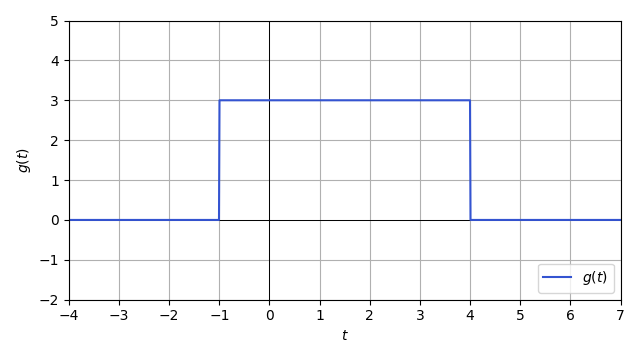
\includegraphics[width=0.7\textwidth]{sources/basic_function.png}
    \caption{График функции $f(t)$ --- исходный сигнал}
\end{figure}
В ходе выполнения задания мы будем искусственно зашумлять функцию $g(t)$ и после этого выполнять жёсткую фильтрацию Фурье-образа зашумлённого сигнала различными методами. Зашумлённый сигнал будет выглядеть так:
$$u(t) = g(t) + b\cdot(\text{rand}(\text{size}(t)) - 0.5) + c\cdot\sin(dt)$$ 
Здесь $\text{rand}(\text{size}(t))$ --- функцию, возвращающая вектор, состоящий из случайных чисел от 0 до 1, той же длины, что и вектор $t$. (Подразумевается, что функции работают как линейные операторы, преобразующие вектор $t$ заданной длины в другой вектор такой же длины.)
% MARK: low-pass
\addsubsection{Убираем высокие частоты}
Начнём с так называемого low-pass фильтра или, по-другому говоря, с \textit{фильтра нижних частот}, который убирает верхние частоты и пропускает нижние. Зададим $c = 0, d = 0$, коэффициент $b$ будет варироваться в множестве $\{0.5, 1.5, 3\}$. Посмотрим, как выглядит зашумлённая функция для каждого $b$:
\begin{figure}[H]
    \begin{minipage}{0.33\textwidth}
        \centering 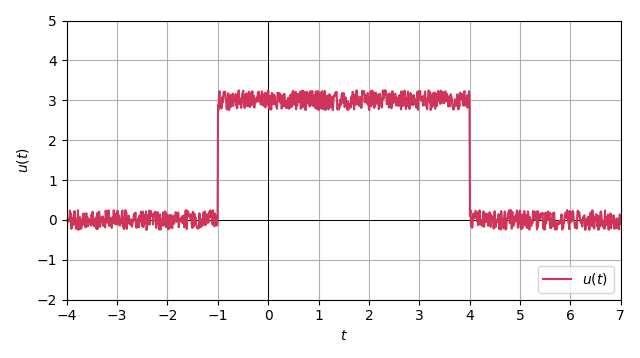
\includegraphics[width=\textwidth]{sources/low-pass filter/noisy (b=0.5).png}
        \caption{$b = 0.5$}
    \end{minipage}\hfill
    \begin{minipage}{0.33\textwidth}
        \centering 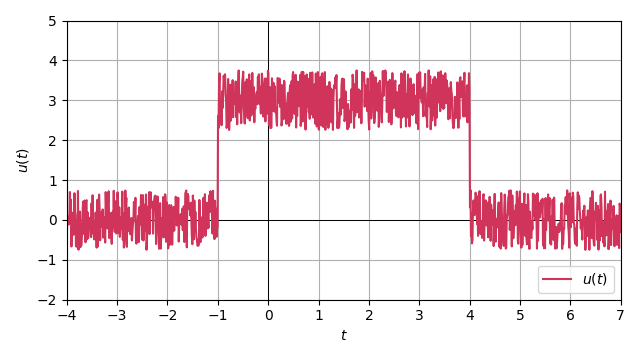
\includegraphics[width=\textwidth]{sources/low-pass filter/noisy (b=1.5).png}
        \caption{$b = 1.5$}
    \end{minipage}\hfill
    \begin{minipage}{0.33\textwidth}
        \centering 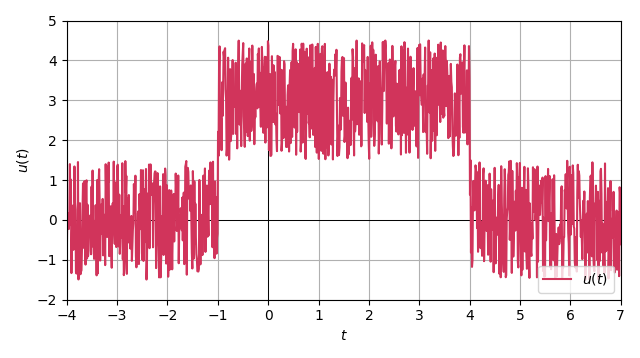
\includegraphics[width=\textwidth]{sources/low-pass filter/noisy (b=3).png}
        \caption{$b = 3$}
    \end{minipage}
    \caption*{Графики функции $u(t)$ --- зашумленный сигнал}
\end{figure}
Приходим к выводу, что с ростом $b$ растёт амплитуда шума в каждой точке сигнала.\newpage
Выберем частоты $v$, за пределами которых мы будем глушить Фурье-образ: $\{3, 7, 13\}$. И для каждого $b$ применим фильтр нижних частот. Предлагаю посмотреть на сравнительные графики модулей Фурье-образов зашумлённого и отфильтрованного сигнала:
\begin{figure}[H]
    \begin{minipage}{0.33\textwidth}
        \centering 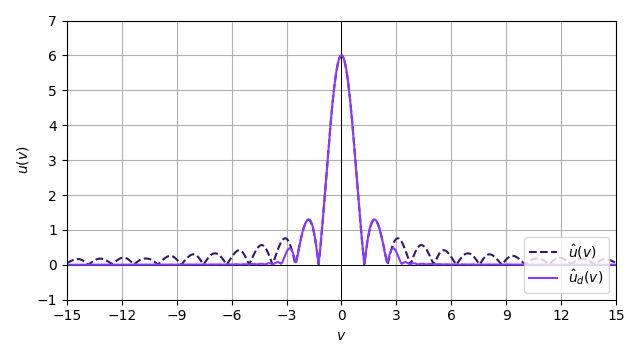
\includegraphics[width=\textwidth]{sources/low-pass filter/fourier (b=0.5, v=3).png}
        \caption{$v = 3$}
    \end{minipage}\hfill
    \begin{minipage}{0.33\textwidth}
        \centering 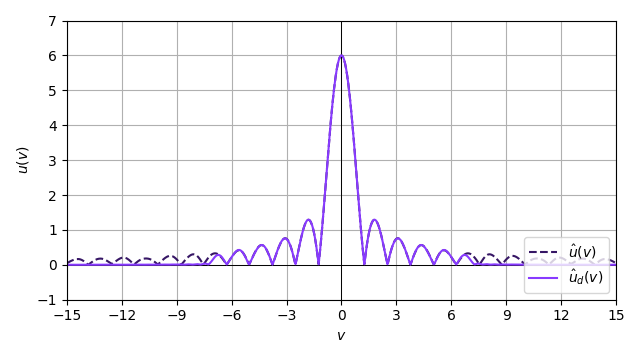
\includegraphics[width=\textwidth]{sources/low-pass filter/fourier (b=0.5, v=7).png}
        \caption{$v = 7$}
    \end{minipage}\hfill
    \begin{minipage}{0.33\textwidth}
        \centering 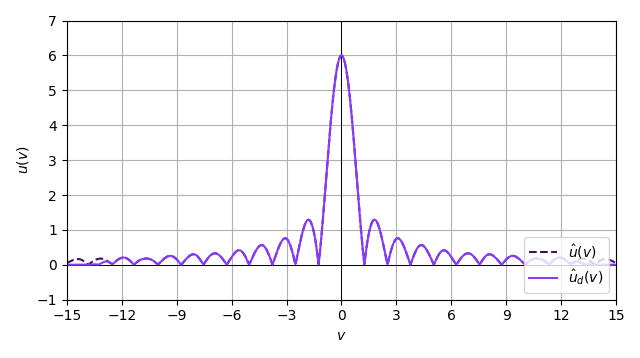
\includegraphics[width=\textwidth]{sources/low-pass filter/fourier (b=0.5, v=13).png}
        \caption{$v = 13$}
    \end{minipage}
    \caption*{Сравнительные графики модулей Фурье-образов при $b=0.5$}
\end{figure}
Выполним обратное преобразование отфильтрованного Фурье-образа, чтобы получить отфильтрованный сигнал. Посмотрим на сравнительные графики исходного и отфильтрованного сигналов:
\begin{figure}[H]
    \begin{minipage}{0.33\textwidth}
        \centering 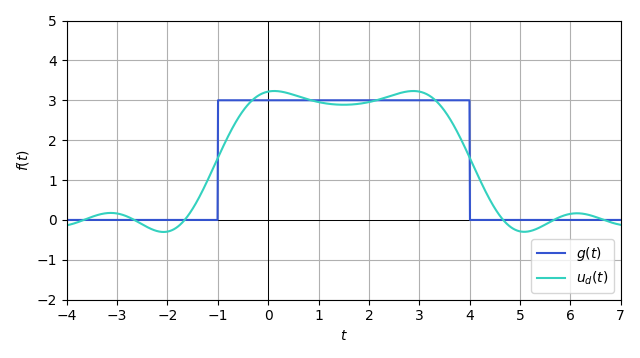
\includegraphics[width=\textwidth]{sources/low-pass filter/denoised (b=0.5, v=3).png}
        \caption{$v = 3$}
    \end{minipage}\hfill
    \begin{minipage}{0.33\textwidth}
        \centering 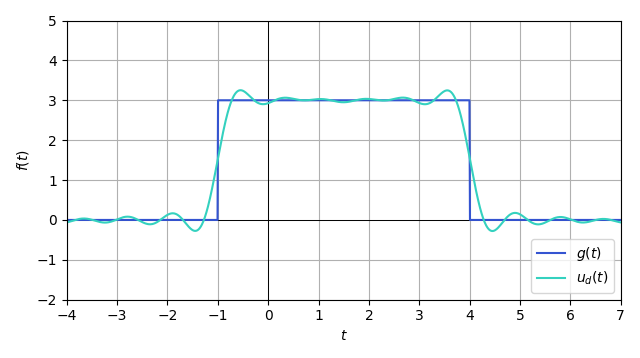
\includegraphics[width=\textwidth]{sources/low-pass filter/denoised (b=0.5, v=7).png}
        \caption{$v = 7$}
    \end{minipage}\hfill
    \begin{minipage}{0.33\textwidth}
        \centering 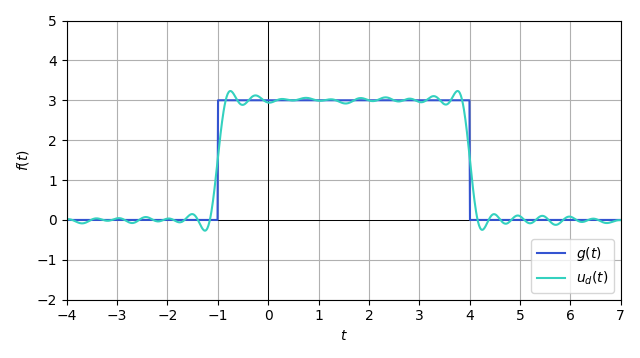
\includegraphics[width=\textwidth]{sources/low-pass filter/denoised (b=0.5, v=13).png}
        \caption{$v = 13$}
    \end{minipage}
    \caption*{Сравнительные графики исходного и отфильтрованного сигналов при $b=0.5$}
\end{figure}
Амплитуда шума невысокая, поэтому не трудно восстановить исходный сигнал, обрезав высокие частоты --- к примеру, на частоте $v = 13$. Отфильтрованный сигнал вполне схож с исходным.\\[0.5em]
Провернём такой же трюк для сигнала с шумом амплитудой $b = 1.5$:
\begin{figure}[H]
    \begin{minipage}{0.33\textwidth}
        \centering 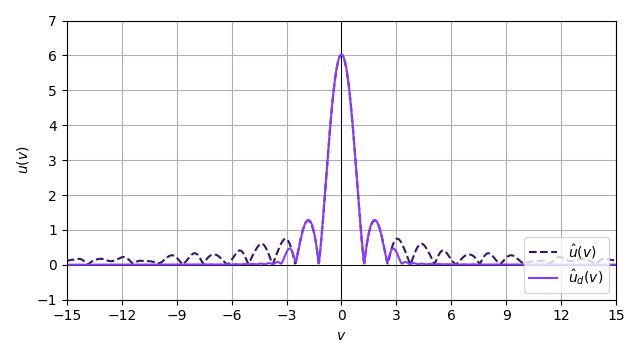
\includegraphics[width=\textwidth]{sources/low-pass filter/fourier (b=1.5, v=3).png}
        \caption{$v = 3$}
    \end{minipage}\hfill
    \begin{minipage}{0.33\textwidth}
        \centering 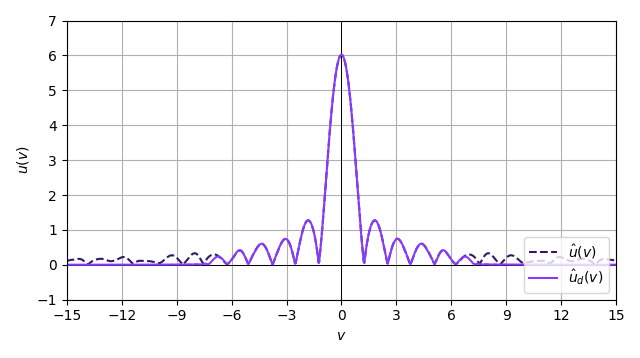
\includegraphics[width=\textwidth]{sources/low-pass filter/fourier (b=1.5, v=7).png}
        \caption{$v = 7$}
    \end{minipage}\hfill
    \begin{minipage}{0.33\textwidth}
        \centering 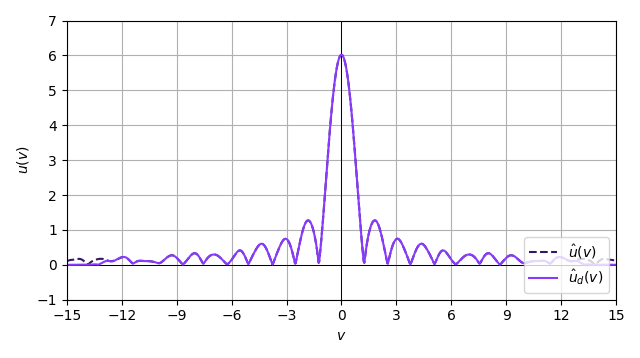
\includegraphics[width=\textwidth]{sources/low-pass filter/fourier (b=1.5, v=13).png}
        \caption{$v = 13$}
    \end{minipage}
    \caption*{Сравнительные графики модулей Фурье-образов при $b=1.5$}
\end{figure}
\begin{figure}[H]
    \begin{minipage}{0.33\textwidth}
        \centering 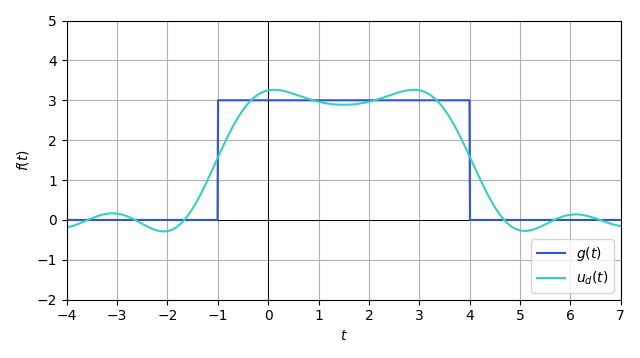
\includegraphics[width=\textwidth]{sources/low-pass filter/denoised (b=1.5, v=3).png}
        \caption{$v = 3$}
    \end{minipage}\hfill
    \begin{minipage}{0.33\textwidth}
        \centering 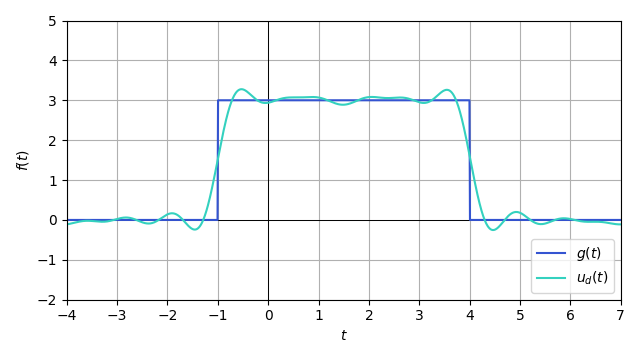
\includegraphics[width=\textwidth]{sources/low-pass filter/denoised (b=1.5, v=7).png}
        \caption{$v = 7$}
    \end{minipage}\hfill
    \begin{minipage}{0.33\textwidth}
        \centering 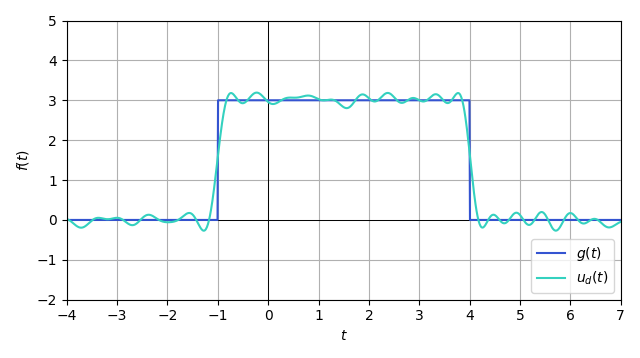
\includegraphics[width=\textwidth]{sources/low-pass filter/denoised (b=1.5, v=13).png}
        \caption{$v = 13$}
    \end{minipage}
    \caption*{Сравнительные графики исходного и отфильтрованного сигналов при $b=1.5$}
\end{figure}
Видим, что исходный сигнал восстановлен не так хорошо, как при $b = 0.5$, но всё равно вполне приемлемо.\\[0.5em]
Наконец, посмотрим на результаты фильтрации для сигнала с амплитудой шума $b = 3$:
\begin{figure}[H]
    \begin{minipage}{0.33\textwidth}
        \centering 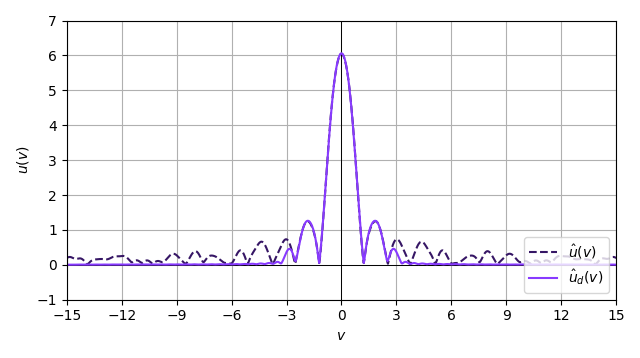
\includegraphics[width=\textwidth]{sources/low-pass filter/fourier (b=3, v=3).png}
        \caption{$v = 3$}
    \end{minipage}\hfill
    \begin{minipage}{0.33\textwidth}
        \centering 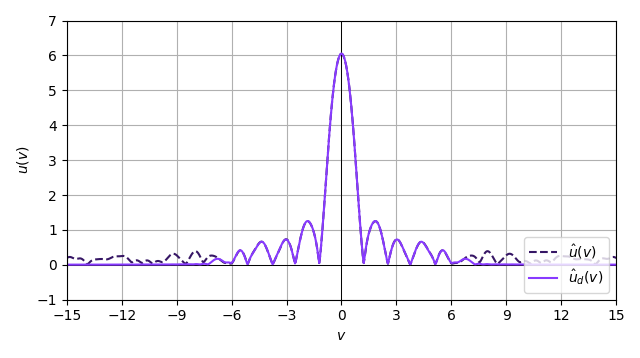
\includegraphics[width=\textwidth]{sources/low-pass filter/fourier (b=3, v=7).png}
        \caption{$v = 7$}
    \end{minipage}\hfill
    \begin{minipage}{0.33\textwidth}
        \centering 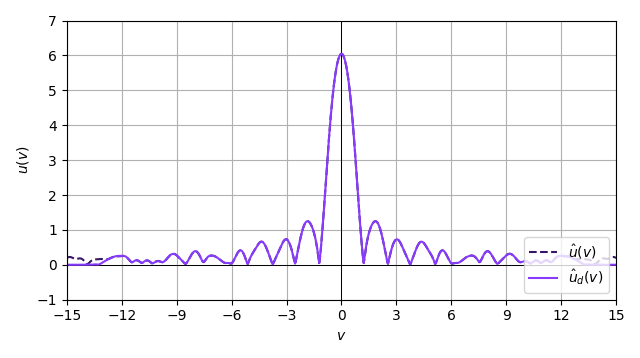
\includegraphics[width=\textwidth]{sources/low-pass filter/fourier (b=3, v=13).png}
        \caption{$v = 13$}
    \end{minipage}
    \caption*{Сравнительные графики модулей Фурье-образов при $b=3$}
\end{figure}
\begin{figure}[H]
    \begin{minipage}{0.33\textwidth}
        \centering 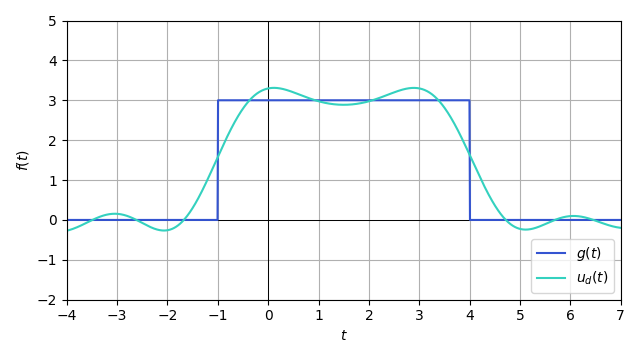
\includegraphics[width=\textwidth]{sources/low-pass filter/denoised (b=3, v=3).png}
        \caption{$v = 3$}
    \end{minipage}\hfill
    \begin{minipage}{0.33\textwidth}
        \centering 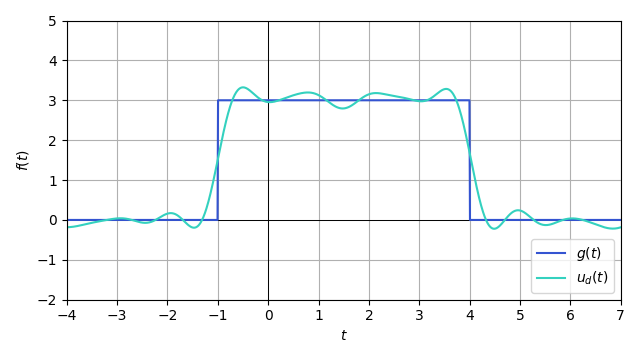
\includegraphics[width=\textwidth]{sources/low-pass filter/denoised (b=3, v=7).png}
        \caption{$v = 7$}
    \end{minipage}\hfill
    \begin{minipage}{0.33\textwidth}
        \centering 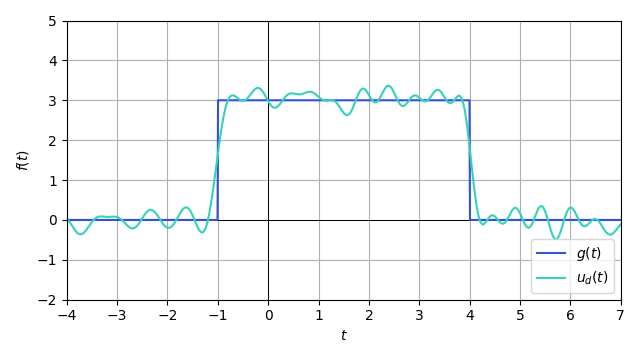
\includegraphics[width=\textwidth]{sources/low-pass filter/denoised (b=3, v=13).png}
        \caption{$v = 13$}
    \end{minipage}
    \caption*{Сравнительные графики исходного и отфильтрованного сигналов при $b=3$}
\end{figure}
Видим, что при $b = 3$ восстановить исходный сигнал становится сложнее, но всё равно возможно. В графике модуля Фурье-образа искажения всё ближе к оси ординат, поэтому приходить выбирать всё меньшую частоту фильтрации $v$, но в таком случае мы теряем всё больше от внешнего облика исходного сигнала.\\[-0.3em]
\begin{quotebox}
    Итак, чем больше $b$ (т.е. чем больше амлитуда шума), тем сложнее восстановить исходный сигнал даже с фильтрацией Фурье-образа. При этом, чем меньше $b$ (т.е. чем меньше шума в сигнале), тем большую частоту фильтрации $v$ можно выбирать, чтобы максимально приблизить отфильтрованный сигнал к исходному.
\end{quotebox}
% MARK: band-stop
\addsubsection{Убираем специфические частоты}
Теперь рассмотрим \textit{band-stop фильтр}, который убирает частоты в определённом диапазоне и пропускает остальные. Зададим набор значений $b = \{0, 1, 2\}$, $c = \{0.8, 1, 1.5\}$ и $d = \{8, 10, 15\}$. Дабы не засорять отчёт множество графиков с полным перебором всех значений (всего $3^3 = 27$ графиков), приведём лишь три примера, репрезентативно отражающих влияние каждого параметра на сигнал:
\begin{figure}[H]
    \begin{minipage}{0.33\textwidth}
        \centering 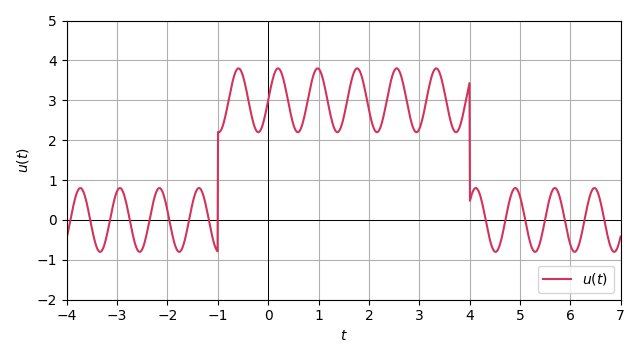
\includegraphics[width=\textwidth]{sources/band-stop filter/noisy (b=0, c=0.8, d=8).png}
        \caption{$b = 0, c = 0.8, d = 8$}
    \end{minipage}\hfill
    \begin{minipage}{0.33\textwidth}
        \centering 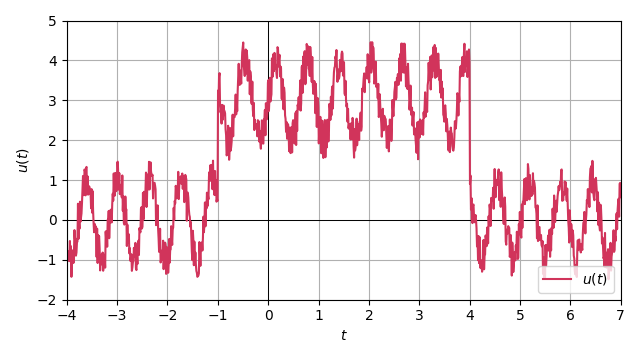
\includegraphics[width=\textwidth]{sources/band-stop filter/noisy (b=1, c=1, d=10).png}
        \caption{$b = 1, c = 1, d = 10$}
    \end{minipage}\hfill
    \begin{minipage}{0.33\textwidth}
        \centering 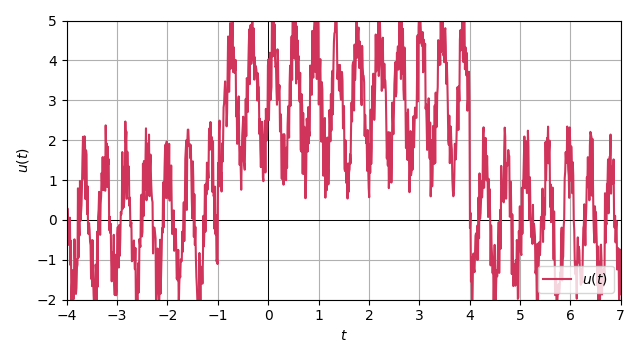
\includegraphics[width=\textwidth]{sources/band-stop filter/noisy (b=2, c=1.5, d=15).png}
        \caption{$b = 2, c = 1.5, d = 15$}
    \end{minipage}
    \caption*{Графики функции $u(t)$ --- зашумленный сигнал}
\end{figure}
Компонента $b$ всё так же отвечает за амплитуду шума, а $c$ и $d$ --- за амплитуду и частоту синусоидального шума. С ростом $c$ увеличивается амплитуда синусоидального шума, а с ростом $d$ --- его частота.\newpage
Выберем частоты $v$, вокруг которых на расстоянии $3$ мы будем глушить Фурье-образ: $\{5, 9, 16\}$. И для каждого набора значений $b, c, d$ применим фильтр. Посмотрим на сравнительные графики модулей Фурье-образов зашумлённого и отфильтрованного сигнала. Примеры будут приведены для тех же наборов, что и выше:
\begin{figure}[H]
    \begin{minipage}{0.33\textwidth}
        \centering 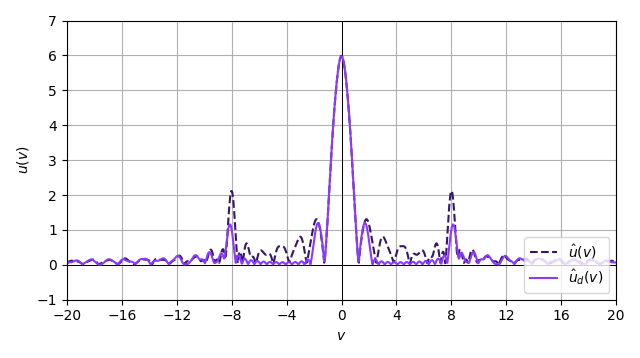
\includegraphics[width=\textwidth]{sources/band-stop filter/fourier (b=0, c=0.8, d=8, v=5).png}
        \caption{$v = 5$}
    \end{minipage}\hfill
    \begin{minipage}{0.33\textwidth}
        \centering 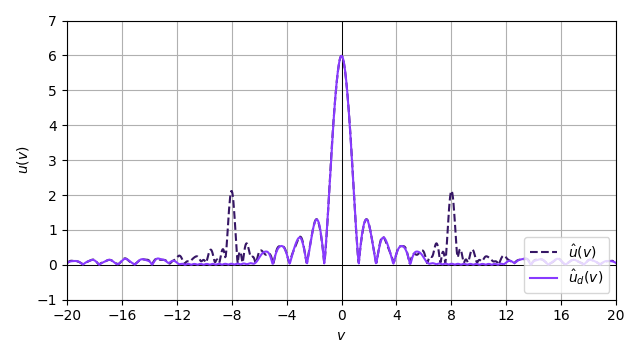
\includegraphics[width=\textwidth]{sources/band-stop filter/fourier (b=0, c=0.8, d=8, v=9).png}
        \caption{$v = 9$}
    \end{minipage}\hfill
    \begin{minipage}{0.33\textwidth}
        \centering 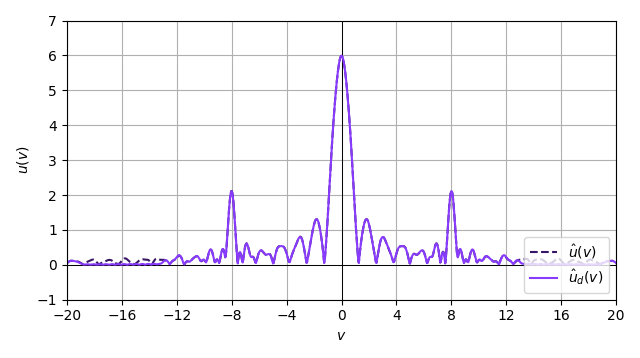
\includegraphics[width=\textwidth]{sources/band-stop filter/fourier (b=0, c=0.8, d=8, v=16).png}
        \caption{$v = 16$}
    \end{minipage}
    \caption*{Сравнительные графики модулей Фурье-образов при $b=0, c=0.8, d=8$}
\end{figure}
Мы наблюдаем ярко выраженную частоту $8$ и $-8$ на графике модуля Фурье-образа, соответствующую частоте синусоидального шума. Взглянем на сравнительные графики исходного и отфильтрованного сигналов:
\begin{figure}[H]
    \begin{minipage}{0.33\textwidth}
        \centering 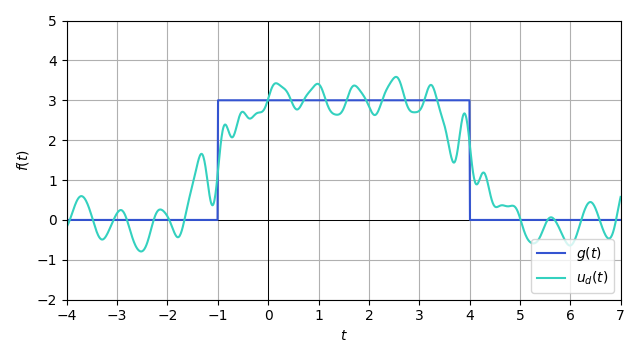
\includegraphics[width=\textwidth]{sources/band-stop filter/denoised (b=0, c=0.8, d=8, v=5).png}
        \caption{$v = 5$}
    \end{minipage}\hfill
    \begin{minipage}{0.33\textwidth}
        \centering 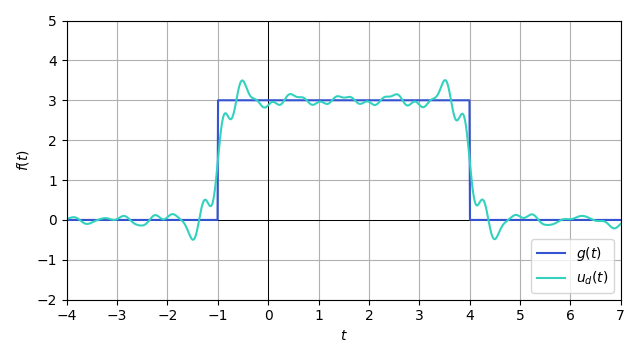
\includegraphics[width=\textwidth]{sources/band-stop filter/denoised (b=0, c=0.8, d=8, v=9).png}
        \caption{$v = 9$}
    \end{minipage}\hfill
    \begin{minipage}{0.33\textwidth}
        \centering 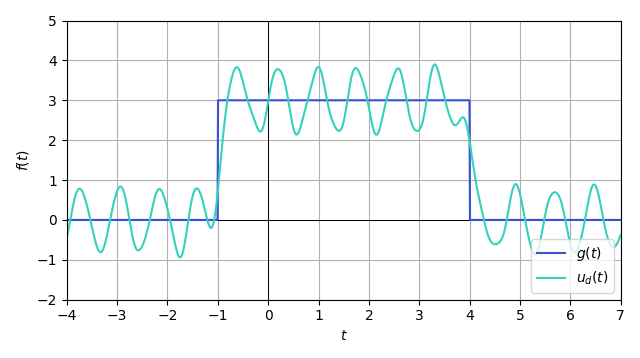
\includegraphics[width=\textwidth]{sources/band-stop filter/denoised (b=0, c=0.8, d=8, v=16).png}
        \caption{$v = 16$}
    \end{minipage}
    \caption*{Сравнительные графики исходного и отфильтрованного сигналов при $b=0, c=0.8, d=8$}
\end{figure}
Действительно, при фильтрации с частотой $v = 9$ мы получаем наиболее чистый сигнал. Для $v = 5$ мы теряем слишком много важной информации, которая хранится в нижних частотах, при этом никак не устраняем случайный и синусоидальный шумы. Для $v = 16$ мы убираем случайный шум, но при этом сохраняем синусоидальный.\\[0.5em]
Посмотрим на результаты фильтрации для сигнала с $b=1, c=1, d=10$:
\begin{figure}[H]
    \begin{minipage}{0.33\textwidth}
        \centering 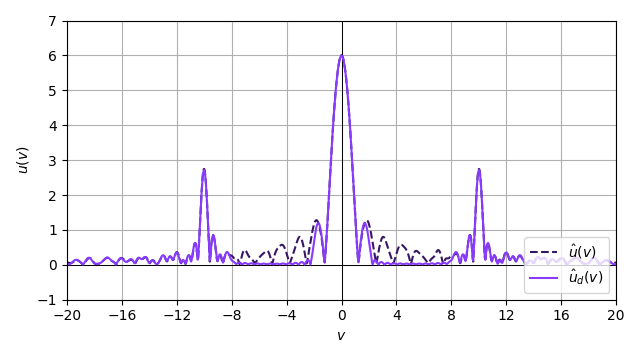
\includegraphics[width=\textwidth]{sources/band-stop filter/fourier (b=1, c=1, d=10, v=5).png}
        \caption{$v = 5$}
    \end{minipage}\hfill
    \begin{minipage}{0.33\textwidth}
        \centering 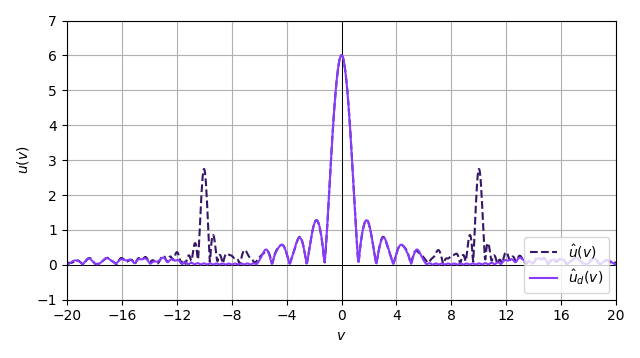
\includegraphics[width=\textwidth]{sources/band-stop filter/fourier (b=1, c=1, d=10, v=9).png}
        \caption{$v = 9$}
    \end{minipage}\hfill
    \begin{minipage}{0.33\textwidth}
        \centering 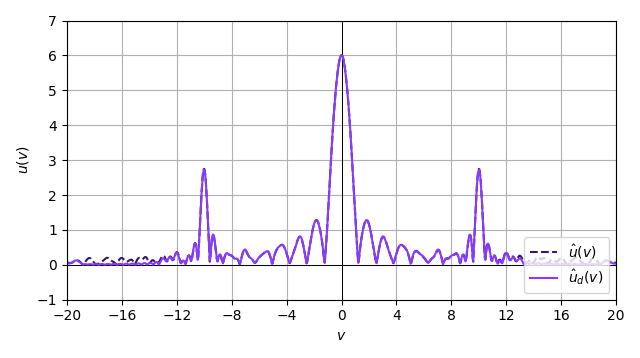
\includegraphics[width=\textwidth]{sources/band-stop filter/fourier (b=1, c=1, d=10, v=16).png}
        \caption{$v = 16$}
    \end{minipage}
    \caption*{Сравнительные графики модулей Фурье-образов при $b=1, c=1, d=10$}
\end{figure}
\begin{figure}[H]
    \begin{minipage}{0.33\textwidth}
        \centering 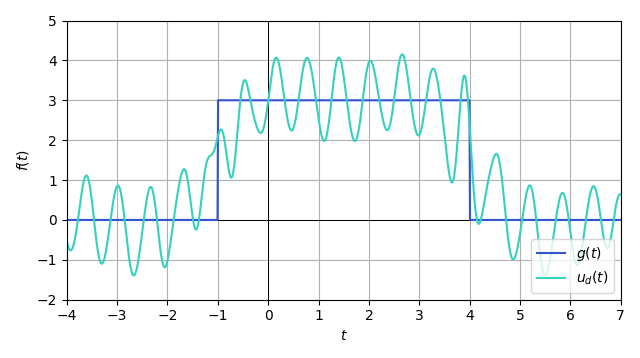
\includegraphics[width=\textwidth]{sources/band-stop filter/denoised (b=1, c=1, d=10, v=5).png}
        \caption{$v = 5$}
    \end{minipage}\hfill
    \begin{minipage}{0.33\textwidth}
        \centering 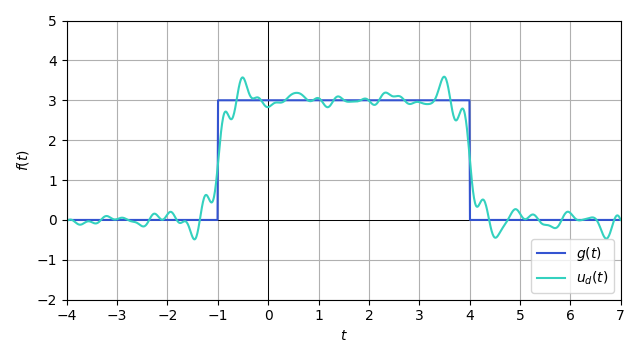
\includegraphics[width=\textwidth]{sources/band-stop filter/denoised (b=1, c=1, d=10, v=9).png}
        \caption{$v = 9$}
    \end{minipage}\hfill
    \begin{minipage}{0.33\textwidth}
        \centering 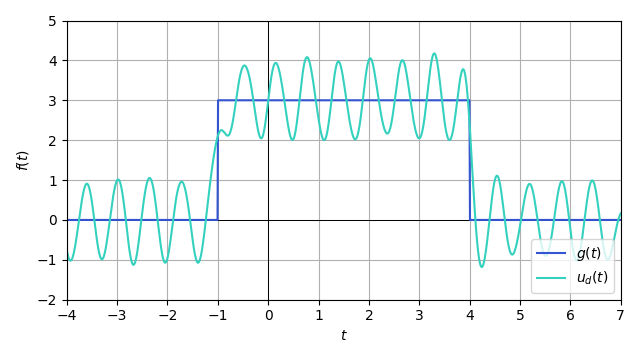
\includegraphics[width=\textwidth]{sources/band-stop filter/denoised (b=1, c=1, d=10, v=16).png}
        \caption{$v = 16$}
    \end{minipage}
    \caption*{Сравнительные графики исходного и отфильтрованного сигналов при $b=1, c=1, d=10$}
\end{figure}
Теперь становится очевидно, что на графике модуля Фурье-образа частота, которую необходимо гасить, равна $d$ и $-d$. При $v = 9$ мы снова получаем чистый сигнал.\\[0.5em]
Наконец, посмотрим на результаты фильтрации для сигнала с $b=2, c=1.5, d=15$:
\begin{figure}[H]
    \begin{minipage}{0.33\textwidth}
        \centering 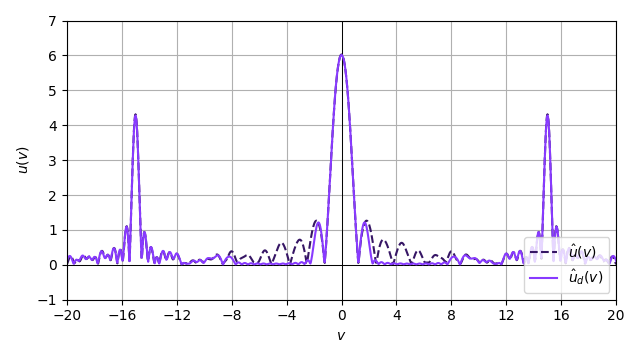
\includegraphics[width=\textwidth]{sources/band-stop filter/fourier (b=2, c=1.5, d=15, v=5).png}
        \caption{$v = 5$}
    \end{minipage}\hfill
    \begin{minipage}{0.33\textwidth}
        \centering 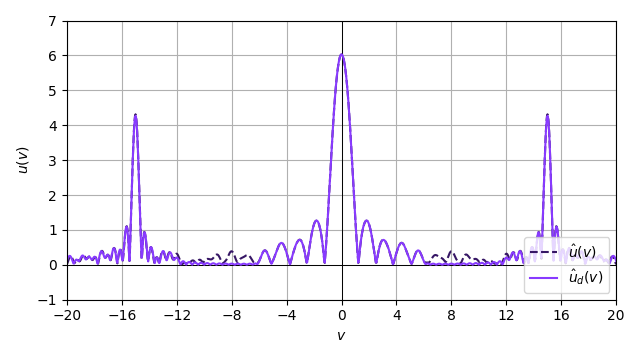
\includegraphics[width=\textwidth]{sources/band-stop filter/fourier (b=2, c=1.5, d=15, v=9).png}
        \caption{$v = 9$}
    \end{minipage}\hfill
    \begin{minipage}{0.33\textwidth}
        \centering 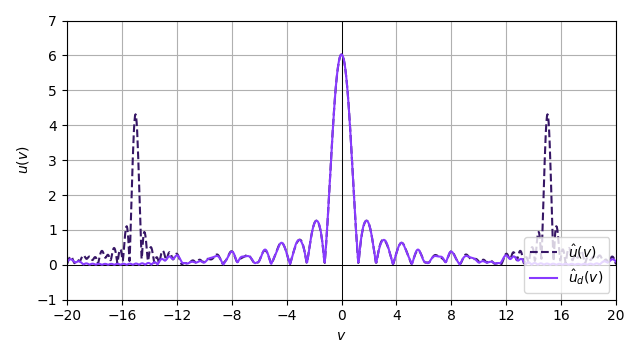
\includegraphics[width=\textwidth]{sources/band-stop filter/fourier (b=2, c=1.5, d=15, v=16).png}
        \caption{$v = 16$}
    \end{minipage}
    \caption*{Сравнительные графики модулей Фурье-образов при $b=2, c=1.5, d=15$}
\end{figure}
\begin{figure}[H]
    \begin{minipage}{0.33\textwidth}
        \centering 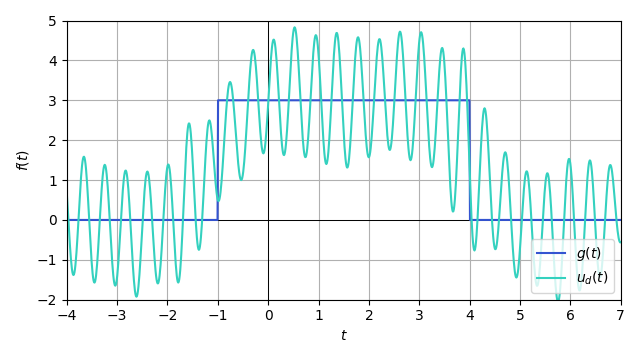
\includegraphics[width=\textwidth]{sources/band-stop filter/denoised (b=2, c=1.5, d=15, v=5).png}
        \caption{$v = 5$}
    \end{minipage}\hfill
    \begin{minipage}{0.33\textwidth}
        \centering 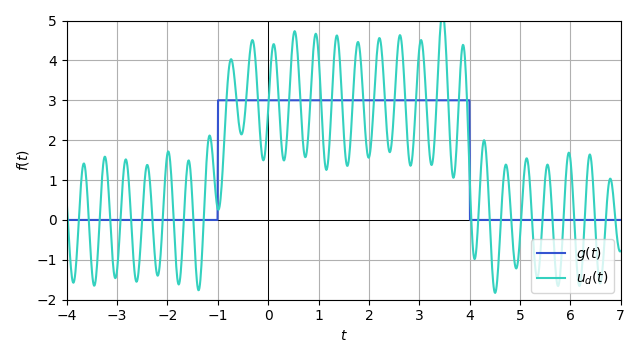
\includegraphics[width=\textwidth]{sources/band-stop filter/denoised (b=2, c=1.5, d=15, v=9).png}
        \caption{$v = 9$}
    \end{minipage}\hfill
    \begin{minipage}{0.33\textwidth}
        \centering 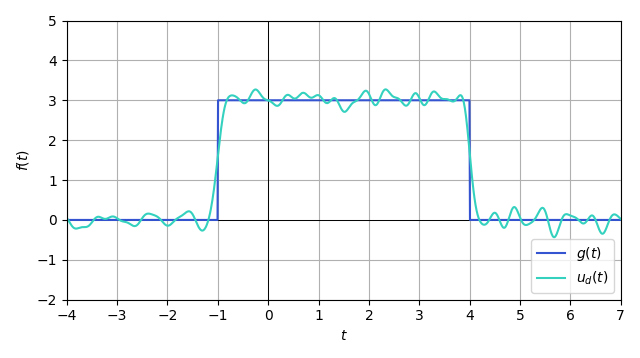
\includegraphics[width=\textwidth]{sources/band-stop filter/denoised (b=2, c=1.5, d=15, v=16).png}
        \caption{$v = 16$}
    \end{minipage}
    \caption*{Сравнительные графики исходного и отфильтрованного сигналов при $b=2, c=1.5, d=15$}
\end{figure}
В этот раз частота синусоидального шума равна $15$ и $-15$, поэтому наиболее чистый сигнал мы получаем при $v = 16$, заодно и фильтруем большую часть случайного шума.\\[-0.3em]
\begin{quotebox}
    Итак, амплитуда синусоидального шума $c$ никак не влияет на фильтрацию и достаточно того, чтобы частота $v$ фильтрации совпадала с частотой синусоидального шума $d$ --- тогда весь синусоидальный шум можно погасить. При этом амплитуда случайного шума $b$ всё так же влияет на сложность восстановления исходного сигнала. Это означает, что если $b=0$, то после фильтрации синусоидального шума мы полностью восстановим исходный сигнал.
\end{quotebox}
% MARK: high-pass
\addsubsection{Убираем низкие частоты?}
Действительно, есть ли смысл гасить нижние частоты? Давайте проверим, рассмотрев \textit{high-pass фильтр}, который убирает низкие частоты и пропускает высокие. Используем тот же набор значений, что и для band-stop фильтра, и те же зашумленные сигналы:
\begin{figure}[H]
    \begin{minipage}{0.33\textwidth}
        \centering 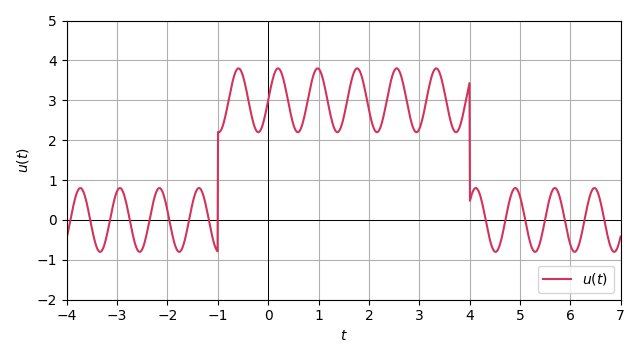
\includegraphics[width=\textwidth]{sources/band-stop filter/noisy (b=0, c=0.8, d=8).png}
        \caption{$b = 0, c = 0.8, d = 8$}
    \end{minipage}\hfill
    \begin{minipage}{0.33\textwidth}
        \centering 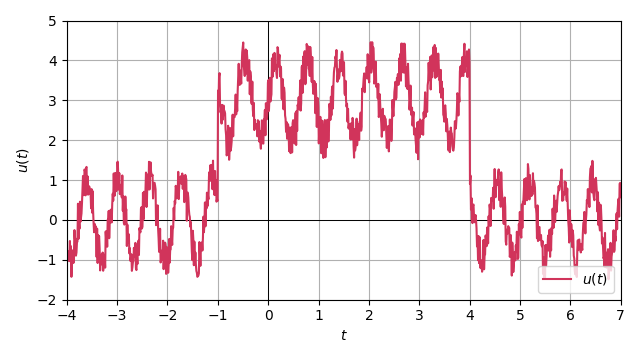
\includegraphics[width=\textwidth]{sources/band-stop filter/noisy (b=1, c=1, d=10).png}
        \caption{$b = 1, c = 1, d = 10$}
    \end{minipage}\hfill
    \begin{minipage}{0.33\textwidth}
        \centering 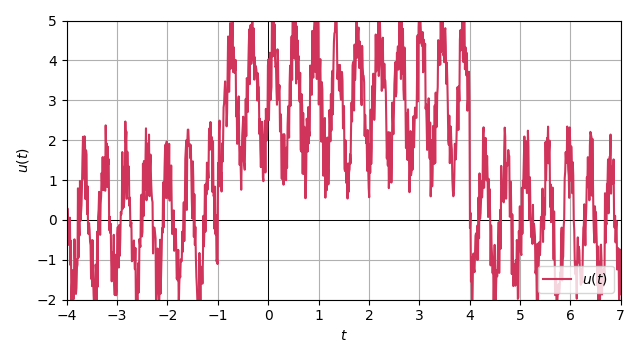
\includegraphics[width=\textwidth]{sources/band-stop filter/noisy (b=2, c=1.5, d=15).png}
        \caption{$b = 2, c = 1.5, d = 15$}
    \end{minipage}
    \caption*{Графики функции $u(t)$ --- зашумленный сигнал}
\end{figure}
Стоит отметить заранее, что на низких частотах хранится вся основная информация о сигнале и его основные компоненты. Поэтому для каждого из сигналов рассмотрим частоты $v$, ниже которых мы будем глушить Фурье-образ: $\{11, 6, 3\}$, но для каждого из сигналов мы выберем по одной частоте $v$ в порядке, представленном выше. Рассмотрим сравнительный график модулеей Фурье-образов зашумлённого и отфильтрованного сигналов:
\begin{figure}[H]
    \begin{minipage}{0.33\textwidth}
        \centering 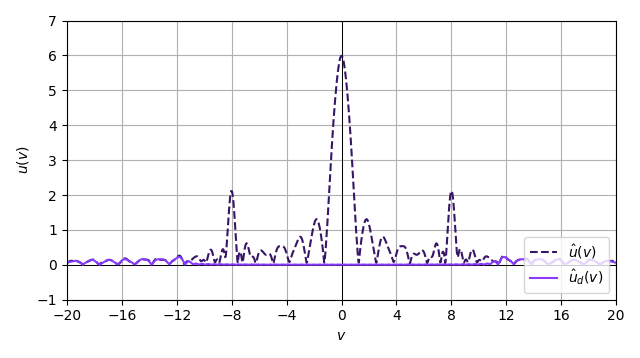
\includegraphics[width=\textwidth]{sources/high-pass filter/fourier (b=0, c=0.8, d=8, v=11).png}
        \caption{$b = 0, c = 0.8, d = 8, v = 11$}
    \end{minipage}\hfill
    \begin{minipage}{0.33\textwidth}
        \centering 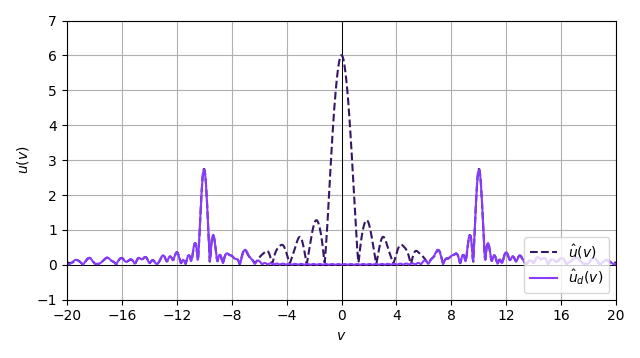
\includegraphics[width=\textwidth]{sources/high-pass filter/fourier (b=1, c=1, d=10, v=6).png}
        \caption{$b = 1, c = 1, d = 10, v = 6$}
    \end{minipage}\hfill
    \begin{minipage}{0.33\textwidth}
        \centering 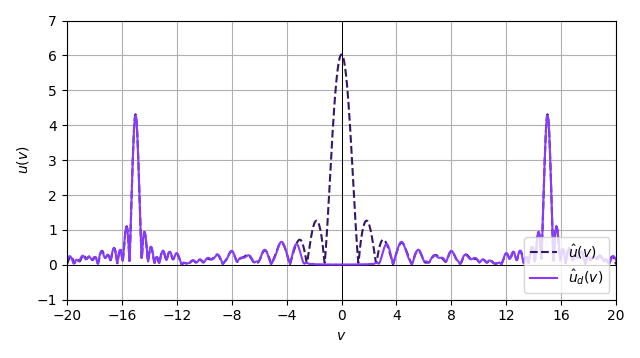
\includegraphics[width=\textwidth]{sources/high-pass filter/fourier (b=2, c=1.5, d=15, v=3).png}
        \caption{$b = 2, c = 1.5, d = 15, v = 3$}
    \end{minipage}
    \caption*{Сравнительные графики модулей Фурье-образов}
\end{figure}
\begin{figure}[H]
    \begin{minipage}{0.33\textwidth}
        \centering 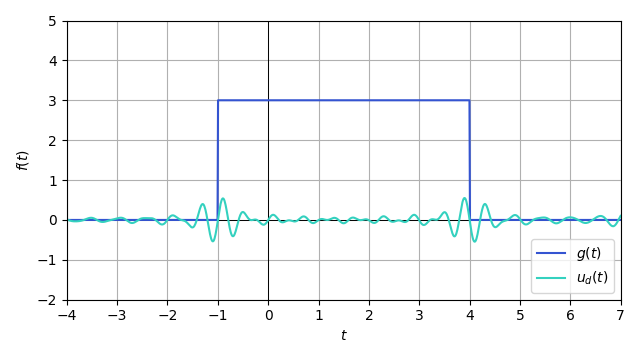
\includegraphics[width=\textwidth]{sources/high-pass filter/denoised (b=0, c=0.8, d=8, v=11).png}
        \caption{$b = 0, c = 0.8, d = 8, v = 11$}
    \end{minipage}\hfill
    \begin{minipage}{0.33\textwidth}
        \centering \includegraphics[width=\textwidth]{sources/high-pass filter/denoised (b=1, c=1, d=10, v=6).png}
        \caption{$b = 1, c = 1, d = 10, v = 6$}
    \end{minipage}\hfill
    \begin{minipage}{0.33\textwidth}
        \centering \includegraphics[width=\textwidth]{sources/high-pass filter/denoised (b=2, c=1.5, d=15, v=3).png}
        \caption{$b = 2, c = 1.5, d = 15, v = 3$}
    \end{minipage}
    \caption*{Сравнительные графики исходного и отфильтрованного сигналов}
\end{figure}
Видим, что при $v = 11$ мы заглушили в сигнале всё, кроме случайного шума. При $v = 6$ мы сохраняем ещё и синусоидальный шум, а при $v = 3$ мы сохраняем всё, кроме основного перепада прямоугольной волны.\\[-0.3em]
\begin{quotebox}
    Итак, гасить низкие частоты в сигнале не имеет смысла, так как именно на них хранится основная информация о сигнале. Поэтому не стоит рассматривать high-pass фильтр в контексте удаления шумов и восстановления исходного сигнала.
\end{quotebox}
% MARK: Задание №2
\newpage\addsection{Задание №2. Фильтрация звука}
В данном задании мы будем фильтровать звуковой сигнал --- мы слышим записанный с микрофона голос и шум в низких частотах. Для этого мы будем использовать библиотеку \texttt{librosa} для чтения и записи аудиофайла, библиотеку \texttt{numpy} для фильтрации Фурье-образа и, как и всегда, \texttt{matplotlib} для отображения графиков.\\[0.5em]
Для начала загрузим аудиофайл и посмотрим на график амплитуды от времени звукового сигнала:
\begin{figure}[H]
    \centering \includegraphics[width=0.7\textwidth]{sources/audio/MUHA.png}
    \caption{График звукового сигнала}
\end{figure}
Теперь применим Фурье-преобразование к сигналу и посмотрим на график модуля Фурье-образа. График сравнительный, то есть здесь отображены Фурье-образы зашумлённого и отфильтрованного сигналов:
\begin{figure}[H]
    \centering \includegraphics[width=0.7\textwidth]{sources/audio/fourier_MUHA.png}
    \caption{График модуля Фурье-образа оригинального и отфильтрованного сигналов}
\end{figure}
Как мы видим, в диапазоне от 0 Гц до 300 Гц наблюдается шум, который заглушает голос. Сам голос находится в диапазоне от 550 Гц до 750 Гц. Но наблюдается также небольшой выброс на частоте 420 Гц. Мы применили фильтр нижних частот на частоты до 300 Гц и band-stop фильтр шириной 50 Гц на частоте 400 Гц, удаляющий частоты в определённом диапазоне --- он заглушит сигнал на частотах 350-450 Гц.\newpage
Применим обратное преобразование Фурье, чтобы получить отфильтрованный звуковой сигнал. Посмотрим на график амплитуды от времени отфильтрованного сигнала:
\begin{figure}[H]
    \centering \includegraphics[width=0.7\textwidth]{sources/audio/MUHA_denoised.png}
    \caption{График отфильтрованного звукового сигнала}
\end{figure}
Как мы видим, теперь на графике чётко виден голос, и остался только синусоидальный шум, который достаточно тих, чтобы не отображаться на графике и не мешать восприятию голоса.
\end{document}